\PassOptionsToPackage{unicode=true}{hyperref} % options for packages loaded elsewhere
\PassOptionsToPackage{hyphens}{url}
%
\documentclass[]{article}
\usepackage{lmodern}
\usepackage{amssymb,amsmath}
\usepackage{ifxetex,ifluatex}
\usepackage{fixltx2e} % provides \textsubscript
\ifnum 0\ifxetex 1\fi\ifluatex 1\fi=0 % if pdftex
  \usepackage[T1]{fontenc}
  \usepackage[utf8]{inputenc}
  \usepackage{textcomp} % provides euro and other symbols
\else % if luatex or xelatex
  \usepackage{unicode-math}
  \defaultfontfeatures{Ligatures=TeX,Scale=MatchLowercase}
\fi
% use upquote if available, for straight quotes in verbatim environments
\IfFileExists{upquote.sty}{\usepackage{upquote}}{}
% use microtype if available
\IfFileExists{microtype.sty}{%
\usepackage[]{microtype}
\UseMicrotypeSet[protrusion]{basicmath} % disable protrusion for tt fonts
}{}
\IfFileExists{parskip.sty}{%
\usepackage{parskip}
}{% else
\setlength{\parindent}{0pt}
\setlength{\parskip}{6pt plus 2pt minus 1pt}
}
\usepackage{hyperref}
\hypersetup{
            pdfborder={0 0 0},
            breaklinks=true}
\urlstyle{same}  % don't use monospace font for urls
\usepackage[margin=1in]{geometry}
\usepackage{longtable,booktabs}
% Fix footnotes in tables (requires footnote package)
\IfFileExists{footnote.sty}{\usepackage{footnote}\makesavenoteenv{longtable}}{}
\usepackage{graphicx,grffile}
\makeatletter
\def\maxwidth{\ifdim\Gin@nat@width>\linewidth\linewidth\else\Gin@nat@width\fi}
\def\maxheight{\ifdim\Gin@nat@height>\textheight\textheight\else\Gin@nat@height\fi}
\makeatother
% Scale images if necessary, so that they will not overflow the page
% margins by default, and it is still possible to overwrite the defaults
% using explicit options in \includegraphics[width, height, ...]{}
\setkeys{Gin}{width=\maxwidth,height=\maxheight,keepaspectratio}
\setlength{\emergencystretch}{3em}  % prevent overfull lines
\providecommand{\tightlist}{%
  \setlength{\itemsep}{0pt}\setlength{\parskip}{0pt}}
\setcounter{secnumdepth}{0}
% Redefines (sub)paragraphs to behave more like sections
\ifx\paragraph\undefined\else
\let\oldparagraph\paragraph
\renewcommand{\paragraph}[1]{\oldparagraph{#1}\mbox{}}
\fi
\ifx\subparagraph\undefined\else
\let\oldsubparagraph\subparagraph
\renewcommand{\subparagraph}[1]{\oldsubparagraph{#1}\mbox{}}
\fi

% set default figure placement to htbp
\makeatletter
\def\fps@figure{htbp}
\makeatother


\date{}

\begin{document}

\hypertarget{project-design-documentation}{%
\section{PROJECT Design
Documentation}\label{project-design-documentation}}

\hypertarget{team-information}{%
\subsection{Team Information}\label{team-information}}

\begin{itemize}
\tightlist
\item
  Team name: Team B++
\item
  Team members

  \begin{itemize}
  \tightlist
  \item
    Ryan Kohn
  \item
    Christopher Johns
  \item
    Ryan Floersch
  \item
    Stone Warren
  \item
    Steven McLeod
  \end{itemize}
\end{itemize}

\hypertarget{executive-summary}{%
\subsection{Executive Summary}\label{executive-summary}}

Web Checkers is a simple web game for playing checkers that Team B++ has
undertaken under the direction of our SWEN 261 professor.

\hypertarget{purpose}{%
\subsubsection{Purpose}\label{purpose}}

Team B++'s purpose with this project is to create an easy to use way for
users to play a game of checkers online. Our most important user groups
are our professor and our TA, who will be the main users of our game and
will expect to have a completely functional, error-free experience.

\hypertarget{glossary-and-acronyms}{%
\subsubsection{Glossary and Acronyms}\label{glossary-and-acronyms}}

\begin{longtable}[]{@{}ll@{}}
\toprule
Term & Definition\tabularnewline
\midrule
\endhead
&\tabularnewline
\bottomrule
\end{longtable}

\hypertarget{requirements}{%
\subsection{Requirements}\label{requirements}}

\begin{itemize}
\tightlist
\item
  The user will be able to sign-in to the player lobby and sign-out when
  done playing.
\item
  The user will be able to start and play checkers games with other
  players.
\item
  The user will be able to follow the rules of Checkers to move pieces
  and play the game.
\item
  The user will be able to enter games in alternate modes, including
  spectator mode and replay mode.
\end{itemize}

\hypertarget{definition-of-mvp}{%
\subsubsection{Definition of MVP}\label{definition-of-mvp}}

For our minimal viable product, the first thing we need is a functional
player lobby that allows players to sign in, out, and start games with
unoccupied players. Secondly, we need to complete all in-game
functionality such that both players are able to play a game of checkers
while following the rules, moving and promoting pieces. Finally, we need
to be able to handle games ending through win conditions or player
resignation and direct players appropriately.

\hypertarget{mvp-features}{%
\subsubsection{MVP Features}\label{mvp-features}}

\begin{itemize}
\tightlist
\item
  Player Sign In/Out - Players will be able to sign in and out of the
  player lobby with a unique username.
\item
  Start Game - Players will be able to start a game with other
  unoccupied players.
\item
  Play Turn - Players will be able to make legal moves during their
  turns, and the game will handle alternating turns as players submit
  their moves.
\item
  Game Ending - Game will recognize and handle win conditions and player
  resignation.
\item
  Piece Movement - Pieces will be movable according to checkers rules,
  including handling simple movement, jump moves, multiple jump moves,
  and king movement.
\item
  Promotion - Pieces will promote themselves to kings when they move to
  the opposite side of the board from where they started.
\end{itemize}

\hypertarget{roadmap-of-enhancements}{%
\subsubsection{Roadmap of Enhancements}\label{roadmap-of-enhancements}}

\begin{itemize}
\tightlist
\item
  Spectate Game - Players will be able to join and leave ongoing games
  as a spectator.
\item
  Game Replays - Finished games will be saved and players can watch
  replays of them.
\end{itemize}

\hypertarget{application-domain}{%
\subsection{Application Domain}\label{application-domain}}

This section describes the application domain.

\begin{figure}
\centering
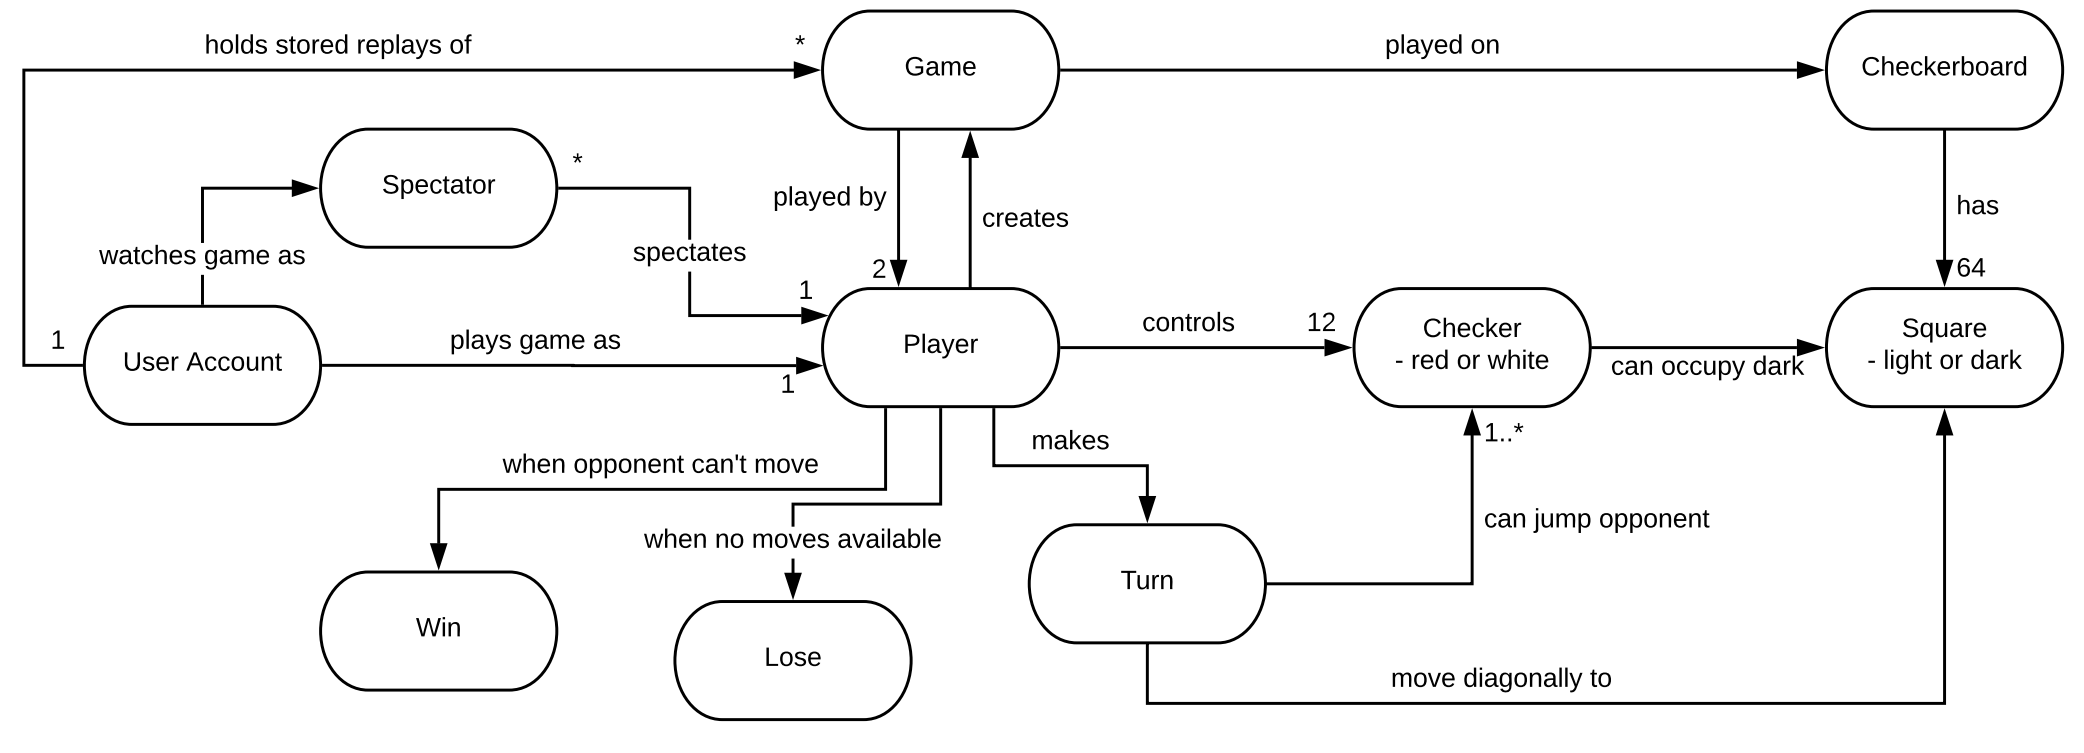
\includegraphics{./tex2pdf.1500/4f3b5fcbfccfe089ecaf165dc9c6e50bfa14e36f.png}
\caption{The WebCheckers Domain Model}
\end{figure}

Users sign in to the application and create a user account. From there,
they start games with other users and become players in those games.
Each game has an 8x8 board made up of light and dark squares and pieces
for each player. Players take turns moving the pieces, and the game ends
when the win/loss conditions are met. Users can also spectate or watch
replays of games rather than play in them.

\hypertarget{architecture-and-design}{%
\subsection{Architecture and Design}\label{architecture-and-design}}

This section describes the application architecture.

\hypertarget{summary}{%
\subsubsection{Summary}\label{summary}}

The following Tiers/Layers model shows a high-level view of the webapp's
architecture.

\begin{figure}
\centering
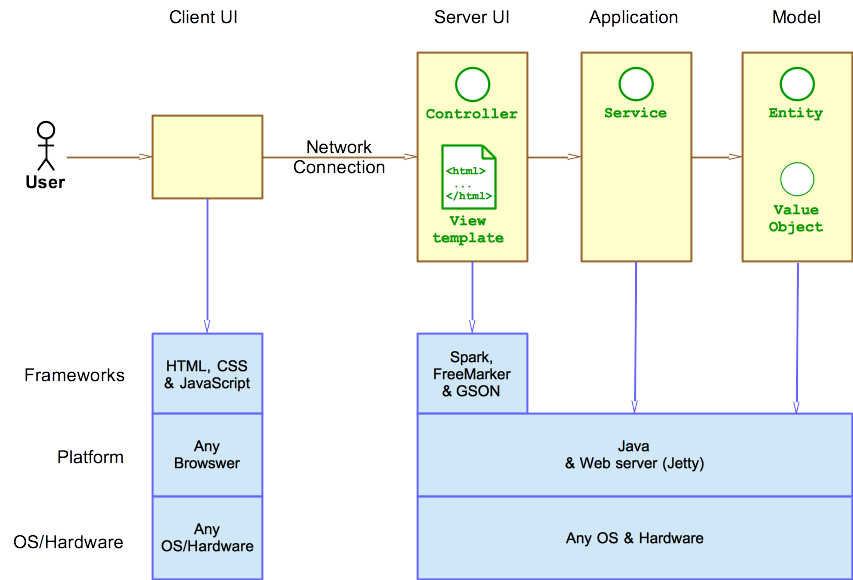
\includegraphics{./tex2pdf.1500/8585463a61d25b331ef215353ef264fe54be55e6.png}
\caption{The Tiers \& Layers of the Architecture}
\end{figure}

As a web application, the user interacts with the system using a
browser. The client-side of the UI is composed of HTML pages with some
minimal CSS for styling the page. There is also some JavaScript that has
been provided to the team by the architect.

The server-side tiers include the UI Tier that is composed of UI
Controllers and Views. Controllers are built using the Spark framework
and View are built using the FreeMarker framework. The Application and
Model tiers are built using plain-old Java objects (POJOs).

Details of the components within these tiers are supplied below.

\hypertarget{overview-of-user-interface}{%
\subsubsection{Overview of User
Interface}\label{overview-of-user-interface}}

This section describes the web interface flow; this is how the user
views and interacts with the WebCheckers application.

\begin{figure}
\centering
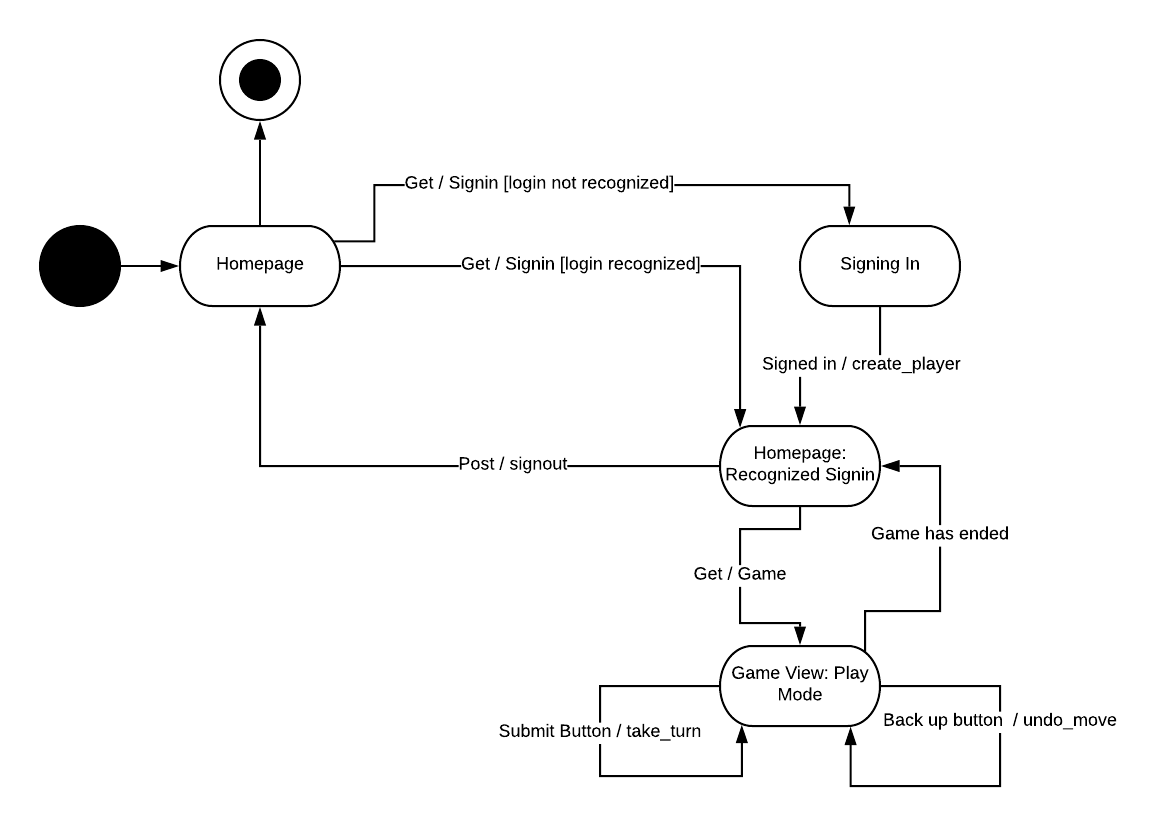
\includegraphics{./tex2pdf.1500/872966d688239a7cc0d12d004f77acfd8041a25f.png}
\caption{The WebCheckers Web Interface Statechart}
\end{figure}

The user will be directed to the home page first. After the user decides
on a username, they will then be directed to a home page that includes
online players.

If the user wants to start a game with someone, they can click on the
players name and if that player is unoccupied both players will be
redirected to a game page.

Once the game has ended, the players are redirected back to the signed
in home page.

\hypertarget{ui-tier}{%
\subsubsection{UI Tier}\label{ui-tier}}

Our UI tier classes consist of different Get and Post Route classes,
including GetGameRoute, GetHomeRoute, GetSignInRoute, PostHomeRoute,
PostSignInRoute, and PostSignOutRoute. These Route classes handle
directing users between the home page, the signed-in homepage, and the
game page. They also give the template engine information on what the
webpage should have/look like.

We also have our WebServer class that initializes the different routes,
as well as Space and Row classes that make up the gameboard interface.

\hypertarget{application-tier}{%
\subsubsection{Application Tier}\label{application-tier}}

The application tier contains our PlayerLobby class, which keeps track
of all players and games, handles sign-ins and outs, and creates new
games.

\hypertarget{model-tier}{%
\subsubsection{Model Tier}\label{model-tier}}

\begin{figure}
\centering
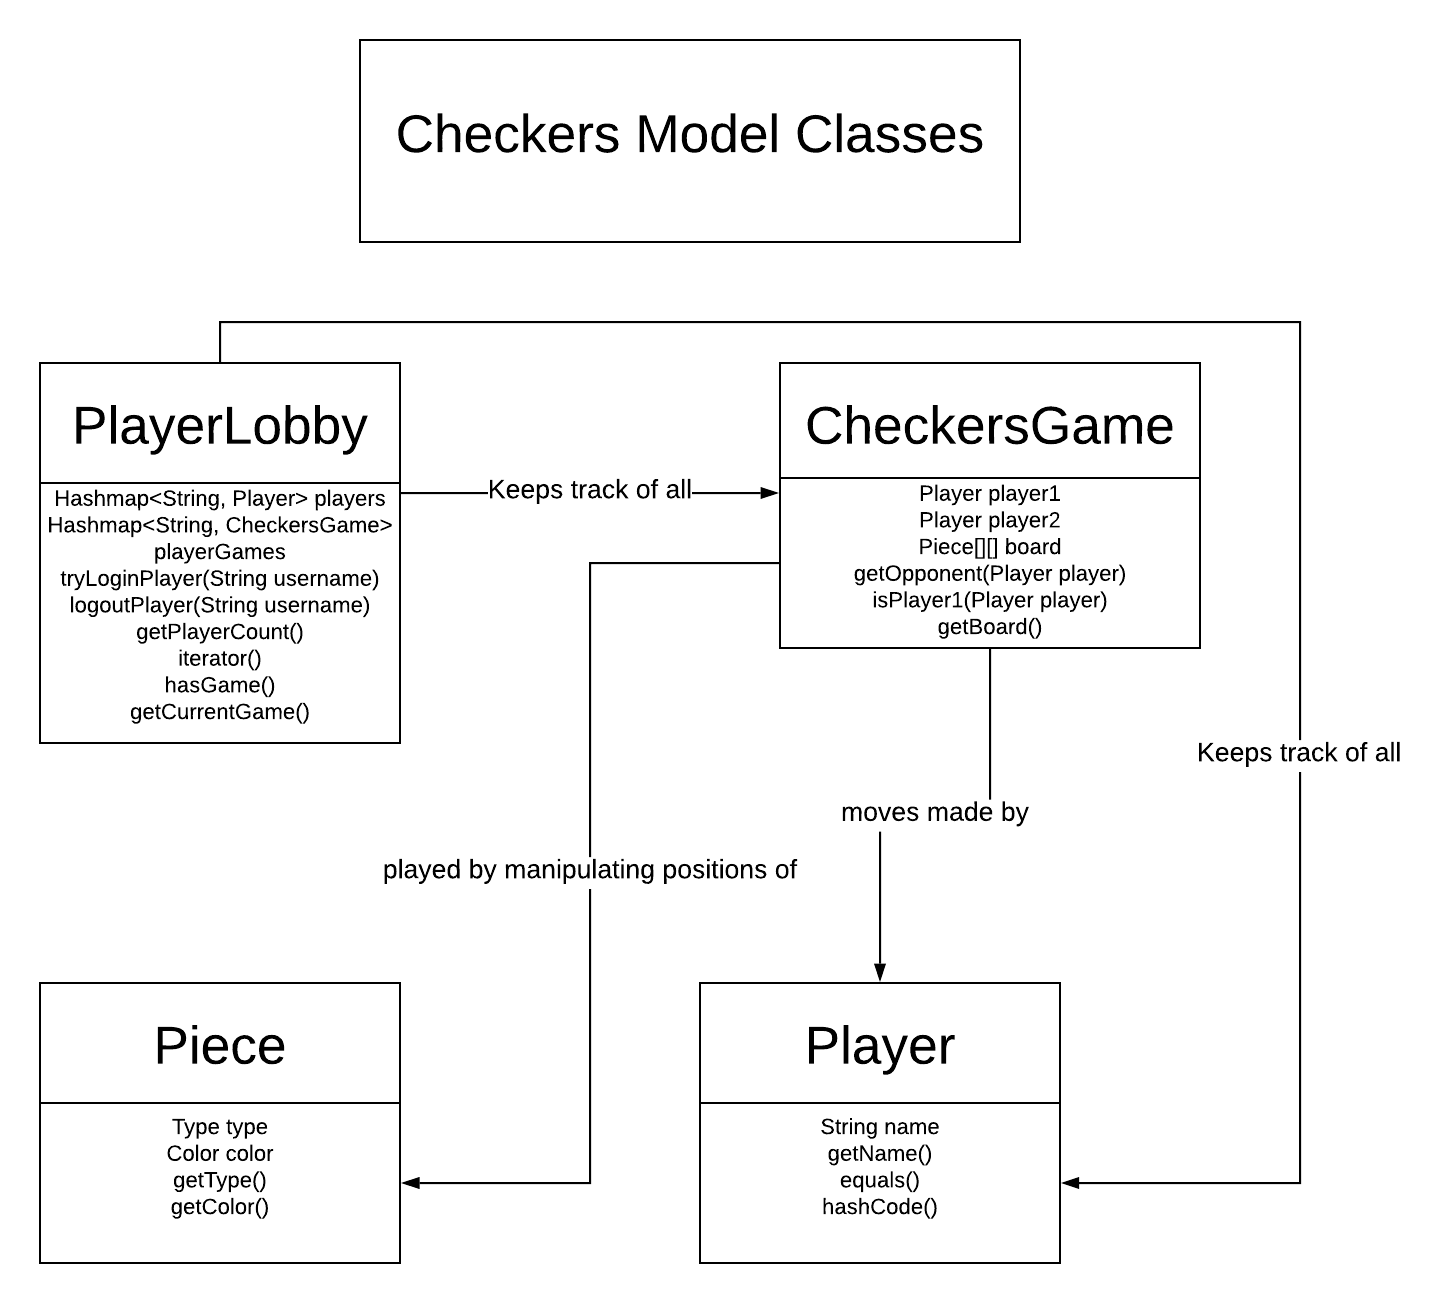
\includegraphics{./tex2pdf.1500/21cc542531619e07b766bad5475800a80e6b8a65.png}
\caption{The WebCheckers Web Model Tier Classes}
\end{figure}

The model tier has a CheckersGame class, which keeps track of an
individual game's players and board state. It also has classes for the
components of the game, including a Piece class, a Player class, and
Type/Color enumerations for the pieces.

\hypertarget{design-improvements}{%
\subsubsection{Design Improvements}\label{design-improvements}}

At this time, we believe that all of our class structures and
relationships are working well for us, and there isn't anything we would
change. This may change after we discover hot spots in our code, or if
we're having trouble creating unit tests.

\hypertarget{testing}{%
\subsection{Testing}\label{testing}}

\hypertarget{acceptance-testing}{%
\subsubsection{Acceptance Testing}\label{acceptance-testing}}

All 18 acceptance criterias for sprint 1 have been met and passed. For
the signin feature there where no problems when testing was done. For
starting the game there where problems when setting up the color of
pieces that appeared on the side of the board. The problem was that the
colors appeared the same for both players, meaning that both players saw
themselves as the red checker pieces For sprint 2 we have 7 user stories
that have not yet been tested.

\hypertarget{unit-testing-and-code-coverage}{%
\subsubsection{Unit Testing and Code
Coverage}\label{unit-testing-and-code-coverage}}

So far our unit testing plan has focused on testing the if the game
exists and if the player has logged in successfully. We plan to test the
players moves next to the such as jumping and moving pieces. We have not
yet done much code coverage yet due to problems that arrised when trying
to use it.

\end{document}
